\part{Hintergrund und Motivation}
\label{part:intro}

\begin{frame}[fragile]{Motivation}
\vspace{10px}
\usebeamerfont{frametitle}\textcolor{blue}{Frage:} \usebeamerfont{text}
\end{frame}

\begin{frame}[fragile]{Struktur des Vortrages}
\begin{itemize}
	\item Hintergründe zur HoloLens, deren Einsatz in der Physik und zum gewählten Experiment
	\item Probleme \& Anforderungen
	\item Lösungsansatz
	\item Umsetzung \& Ergebnisse
	\item Diskussion
\end{itemize}
\end{frame}

\part{HoloLens}
\label{part:hololens}
\begin{frame}[fragile]{}
\begin{figure}[h!]
	\centering
	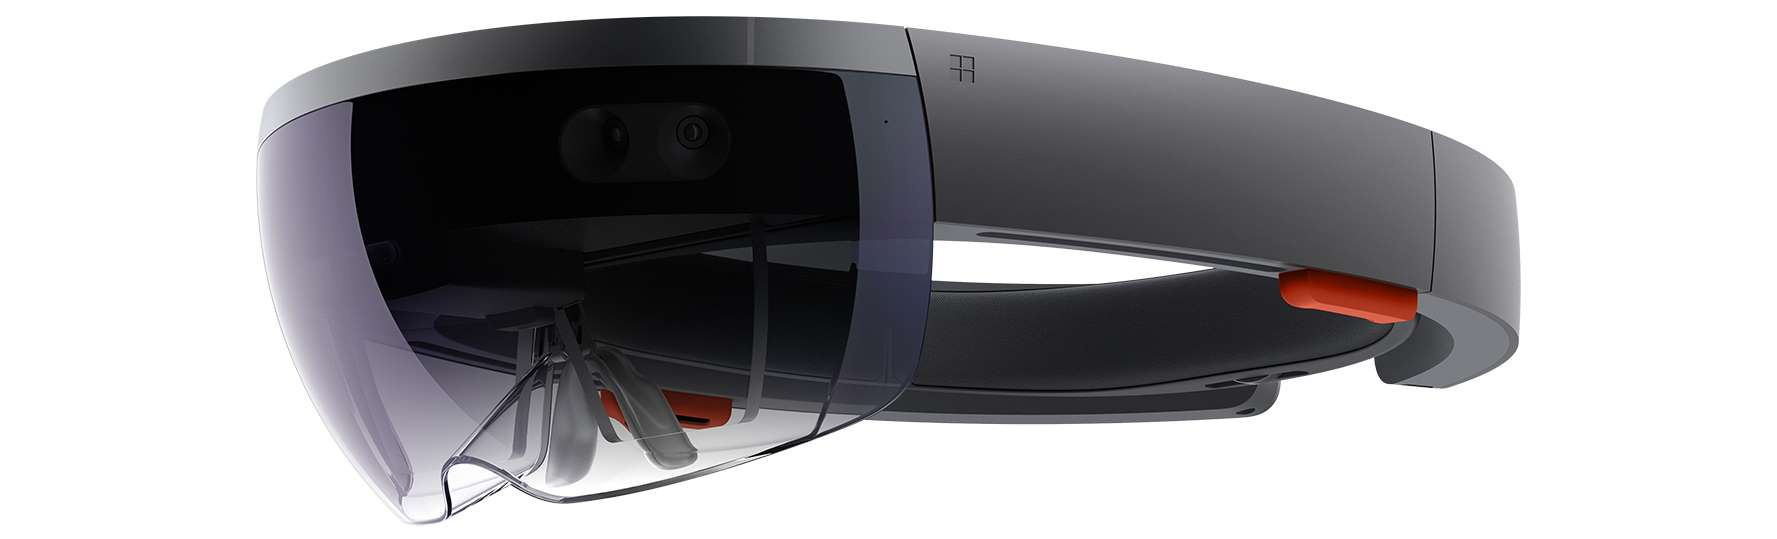
\includegraphics[width=0.7\textwidth]{images/papers/hololens.jpg}
\end{figure}
\begin{itemize}
	\item Projeziert virtuelle Objekte in das Sichtfeld des Nutzers
	\item Nutzer bewegt sich simultan durch reale und virtuelle Szene
	\item Genaue Bestimmung von Position und Ausrichtung im Raum durch Sensoren: \textit{Inside-Out-Tracking}
	\item Interaktion über Gesten und Sprache
	\item Ermöglicht \textit{Augmented Reality} Anwendungen
\end{itemize}	
\end{frame}

\begin{frame}[fragile]{Technische Aspekte}
		\begin{itemize}
			\item \textit{See-Through Display}, Zwei 16:9 HD Bilder, 32\degree FoV (diagonal)
			\begin{itemize}[topsep=-5px]
				\setlength{\itemsep}{-5px}
				\item Einfluss auf Größe und Farbe von Objekten
			\end{itemize}
			\pause
			\item Akkomodation der Augen fest bei 2 m
			\begin{itemize}[topsep=-5px]
				\setlength{\itemsep}{-5px}
				\item Einfluss auf Distanz
			\end{itemize}
			\item \textit{Inside-Out Tracking} über Tiefenkamera, Stereo-Kameras und IMU
			\begin{itemize}[topsep=-5px]
				\setlength{\itemsep}{-5px}
				\item Einfluss auf Positionierung und Stabilität
			\end{itemize}
			\pause
			\item Stand-Alone Device, 1 GHz CPU/HPU, 2 GB RAM
			\begin{itemize}[topsep=-5px]
				\setlength{\itemsep}{-5px}
				\item Einfluss auf Performance
			\end{itemize}
		\end{itemize}
\end{frame}

\part{State of the Art}
\label{part:sota}
\begin{frame}[fragile]{HoloLens in der Physik}
\vspace{0.1cm}
\begin{figure}
	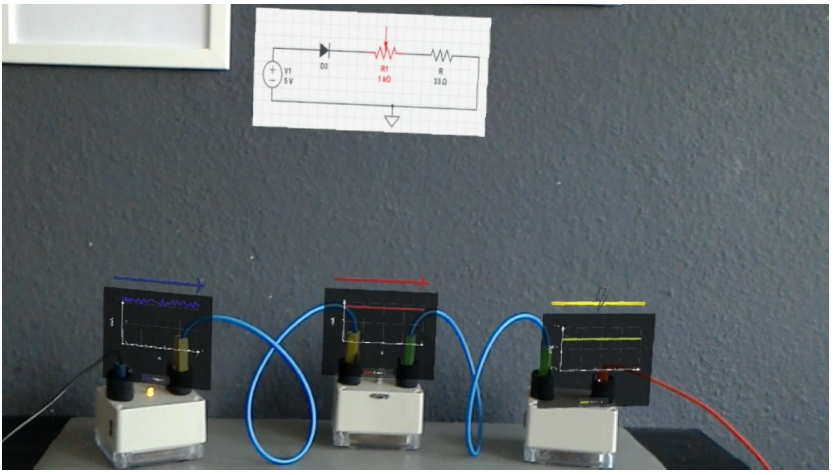
\includegraphics[width=0.42\textwidth]{images/papers/Amiraslanov18.png}
	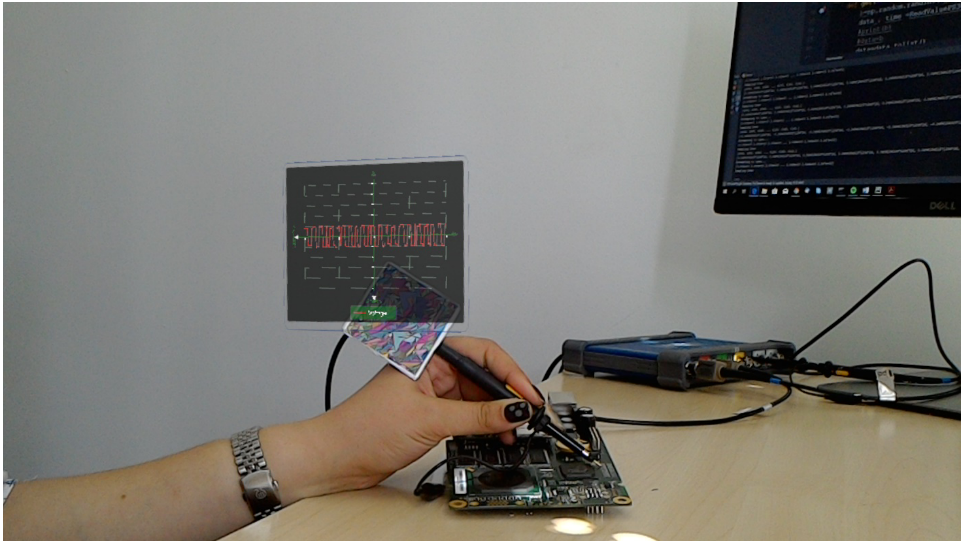
\includegraphics[width=0.42\textwidth]{images/papers/Javaheri18.png}
	\begin{center}
	\vspace{0.03cm}
	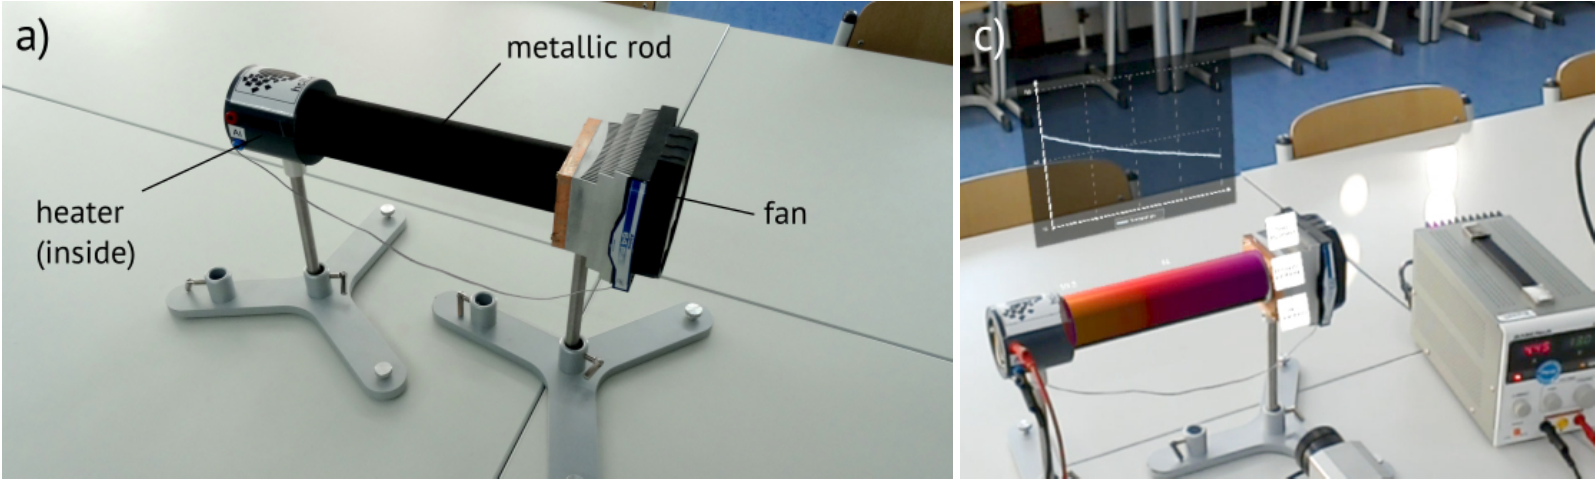
\includegraphics[width=0.85\textwidth]{images/papers/Strzys18.png}	
	\end{center}
	\setlength{\abovecaptionskip}{7pt plus 5pt minus 2pt}
	\caption*{Oben Links: Amiraslanov (2018), Oben Rechts: Javaheri (2018), Unten: Strzys (2018)}
\end{figure}
\end{frame}

\begin{frame}[fragile]{Augmented Reality in der Physik}
	\vspace{0.1cm}
\begin{figure}
	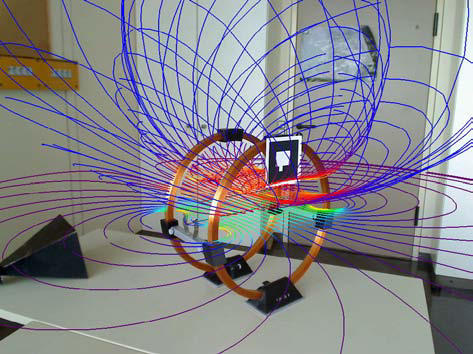
\includegraphics[width=0.32\textwidth]{images/papers/Buchau09.jpg}
	\hspace{0.05cm}
	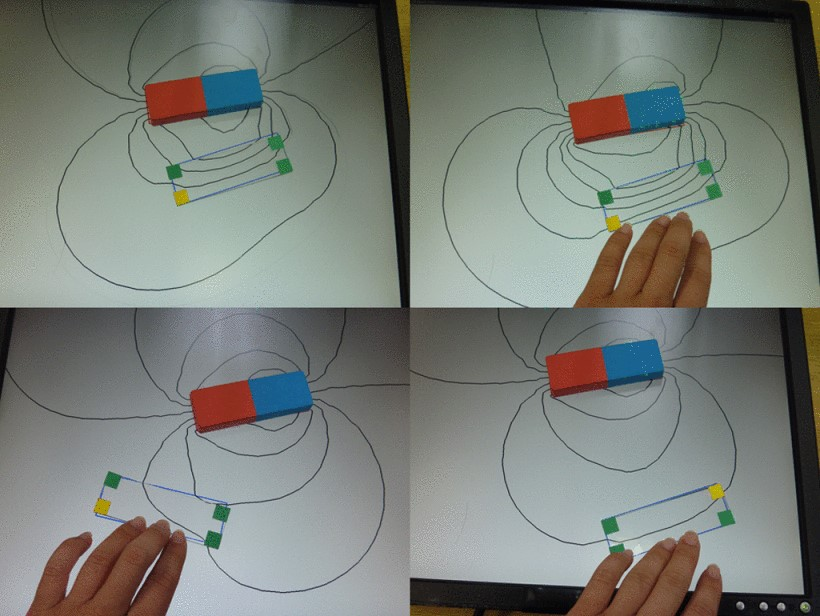
\includegraphics[width=0.32\textwidth]{images/papers/Matsutomo13.jpg}

%	\centering
	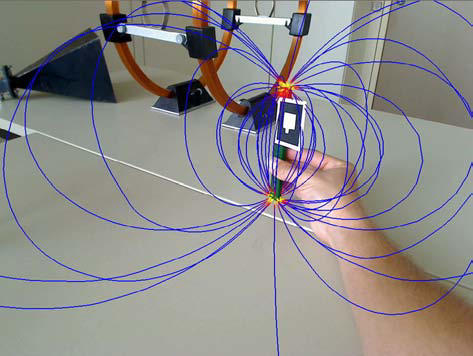
\includegraphics[width=0.32\textwidth]{images/papers/Buchau09_Magnet.jpg}
	\hspace{0.05cm}
	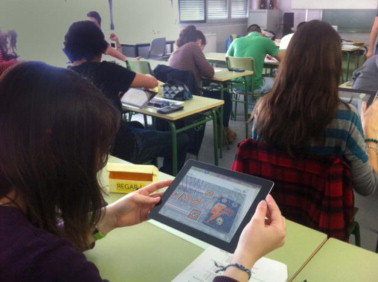
\includegraphics[width=0.32\textwidth]{images/papers/Ibanez14.jpg}

	\setlength{\abovecaptionskip}{7pt plus 5pt minus 2pt}
	\caption*{Links: Buchau (2009), Rechts Oben: Matsutomo (2013), Rechts Unten: Ibanez (2014)}
\end{figure}
\end{frame}

\part{Anwendungsfall: Helmholtz-Spulen}
\label{part:physics}
\begin{frame}[fragile]{Physikalischer Hintergrund}
\begin{minipage}{0.5\textwidth}
	{\setstretch{1.0}
		\begin{itemize}[itemsep=1mm]
			\item Magnetfeld ist 3D-Vektorfeld, Flussdichte $\vec{B}$ in Tesla
			\item Stromfluss durch Spule erzeugt ein Magnetfeld, abhängig von Stromstärke
			\item Helmholtz-Spule: Feld im Inneren weitgehend \textit{homogen}
			\item Feldlinien und Vektormodell sind etablierte Darstellungsmodelle
		\end{itemize}
	}
\end{minipage}
\begin{minipage}{0.45\textwidth}
	\centering
	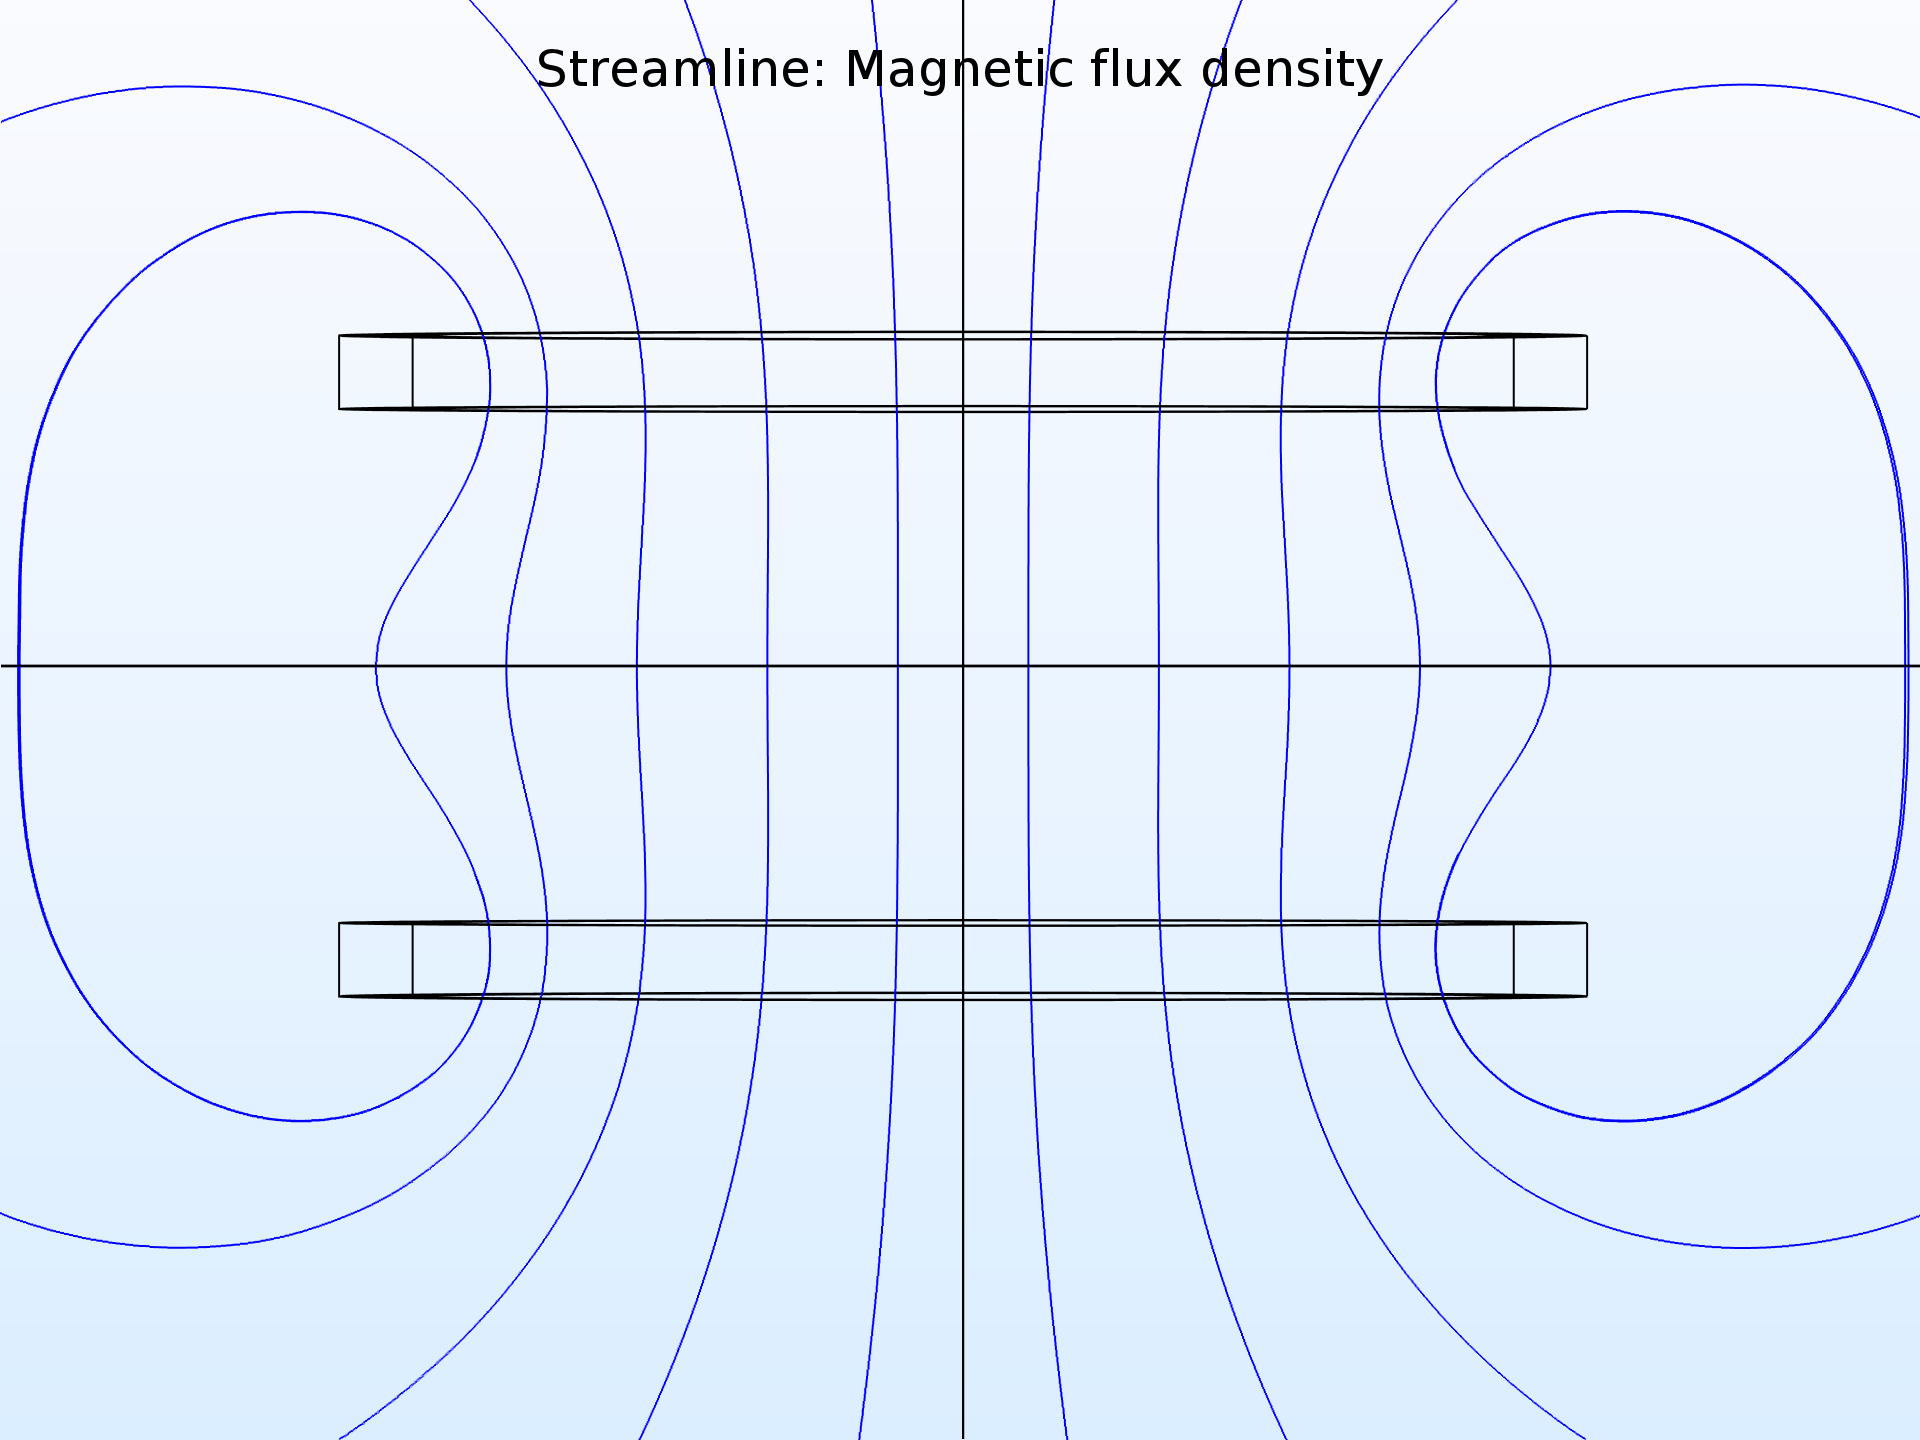
\includegraphics[width=0.9\textwidth]{images/papers/hh_mfield_nocol.png}\\
	\small Darstellung des Magnetfeldes einer Helmholtz-Spule mittels Feldlinien für eine Ebene.
\end{minipage}
\end{frame}
\begin{frame}[fragile]{Experiment: Bestimmung des Erdmagnetfeldes}
\begin{minipage}{0.5\textwidth}
	{\setstretch{1.0}
\begin{itemize}[itemsep=1mm]
	\item[$1.$] Kompass ausrichten lassen
	\item[$2.$] Spule orthogonal zur Nord-Süd-Achse aufstellen
	\item[$3.$] Spannungsquelle einschalten und Stromfluss erhöhen, bis Kompassnadel um 45\degree ausgelenkt ist
	\item[$4.$] Flussdichte mit Formel aus Stromstärke und Spuleneigenschaften berechnen
\end{itemize}
}
\end{minipage}
\begin{minipage}{0.45\textwidth}
	\centering
	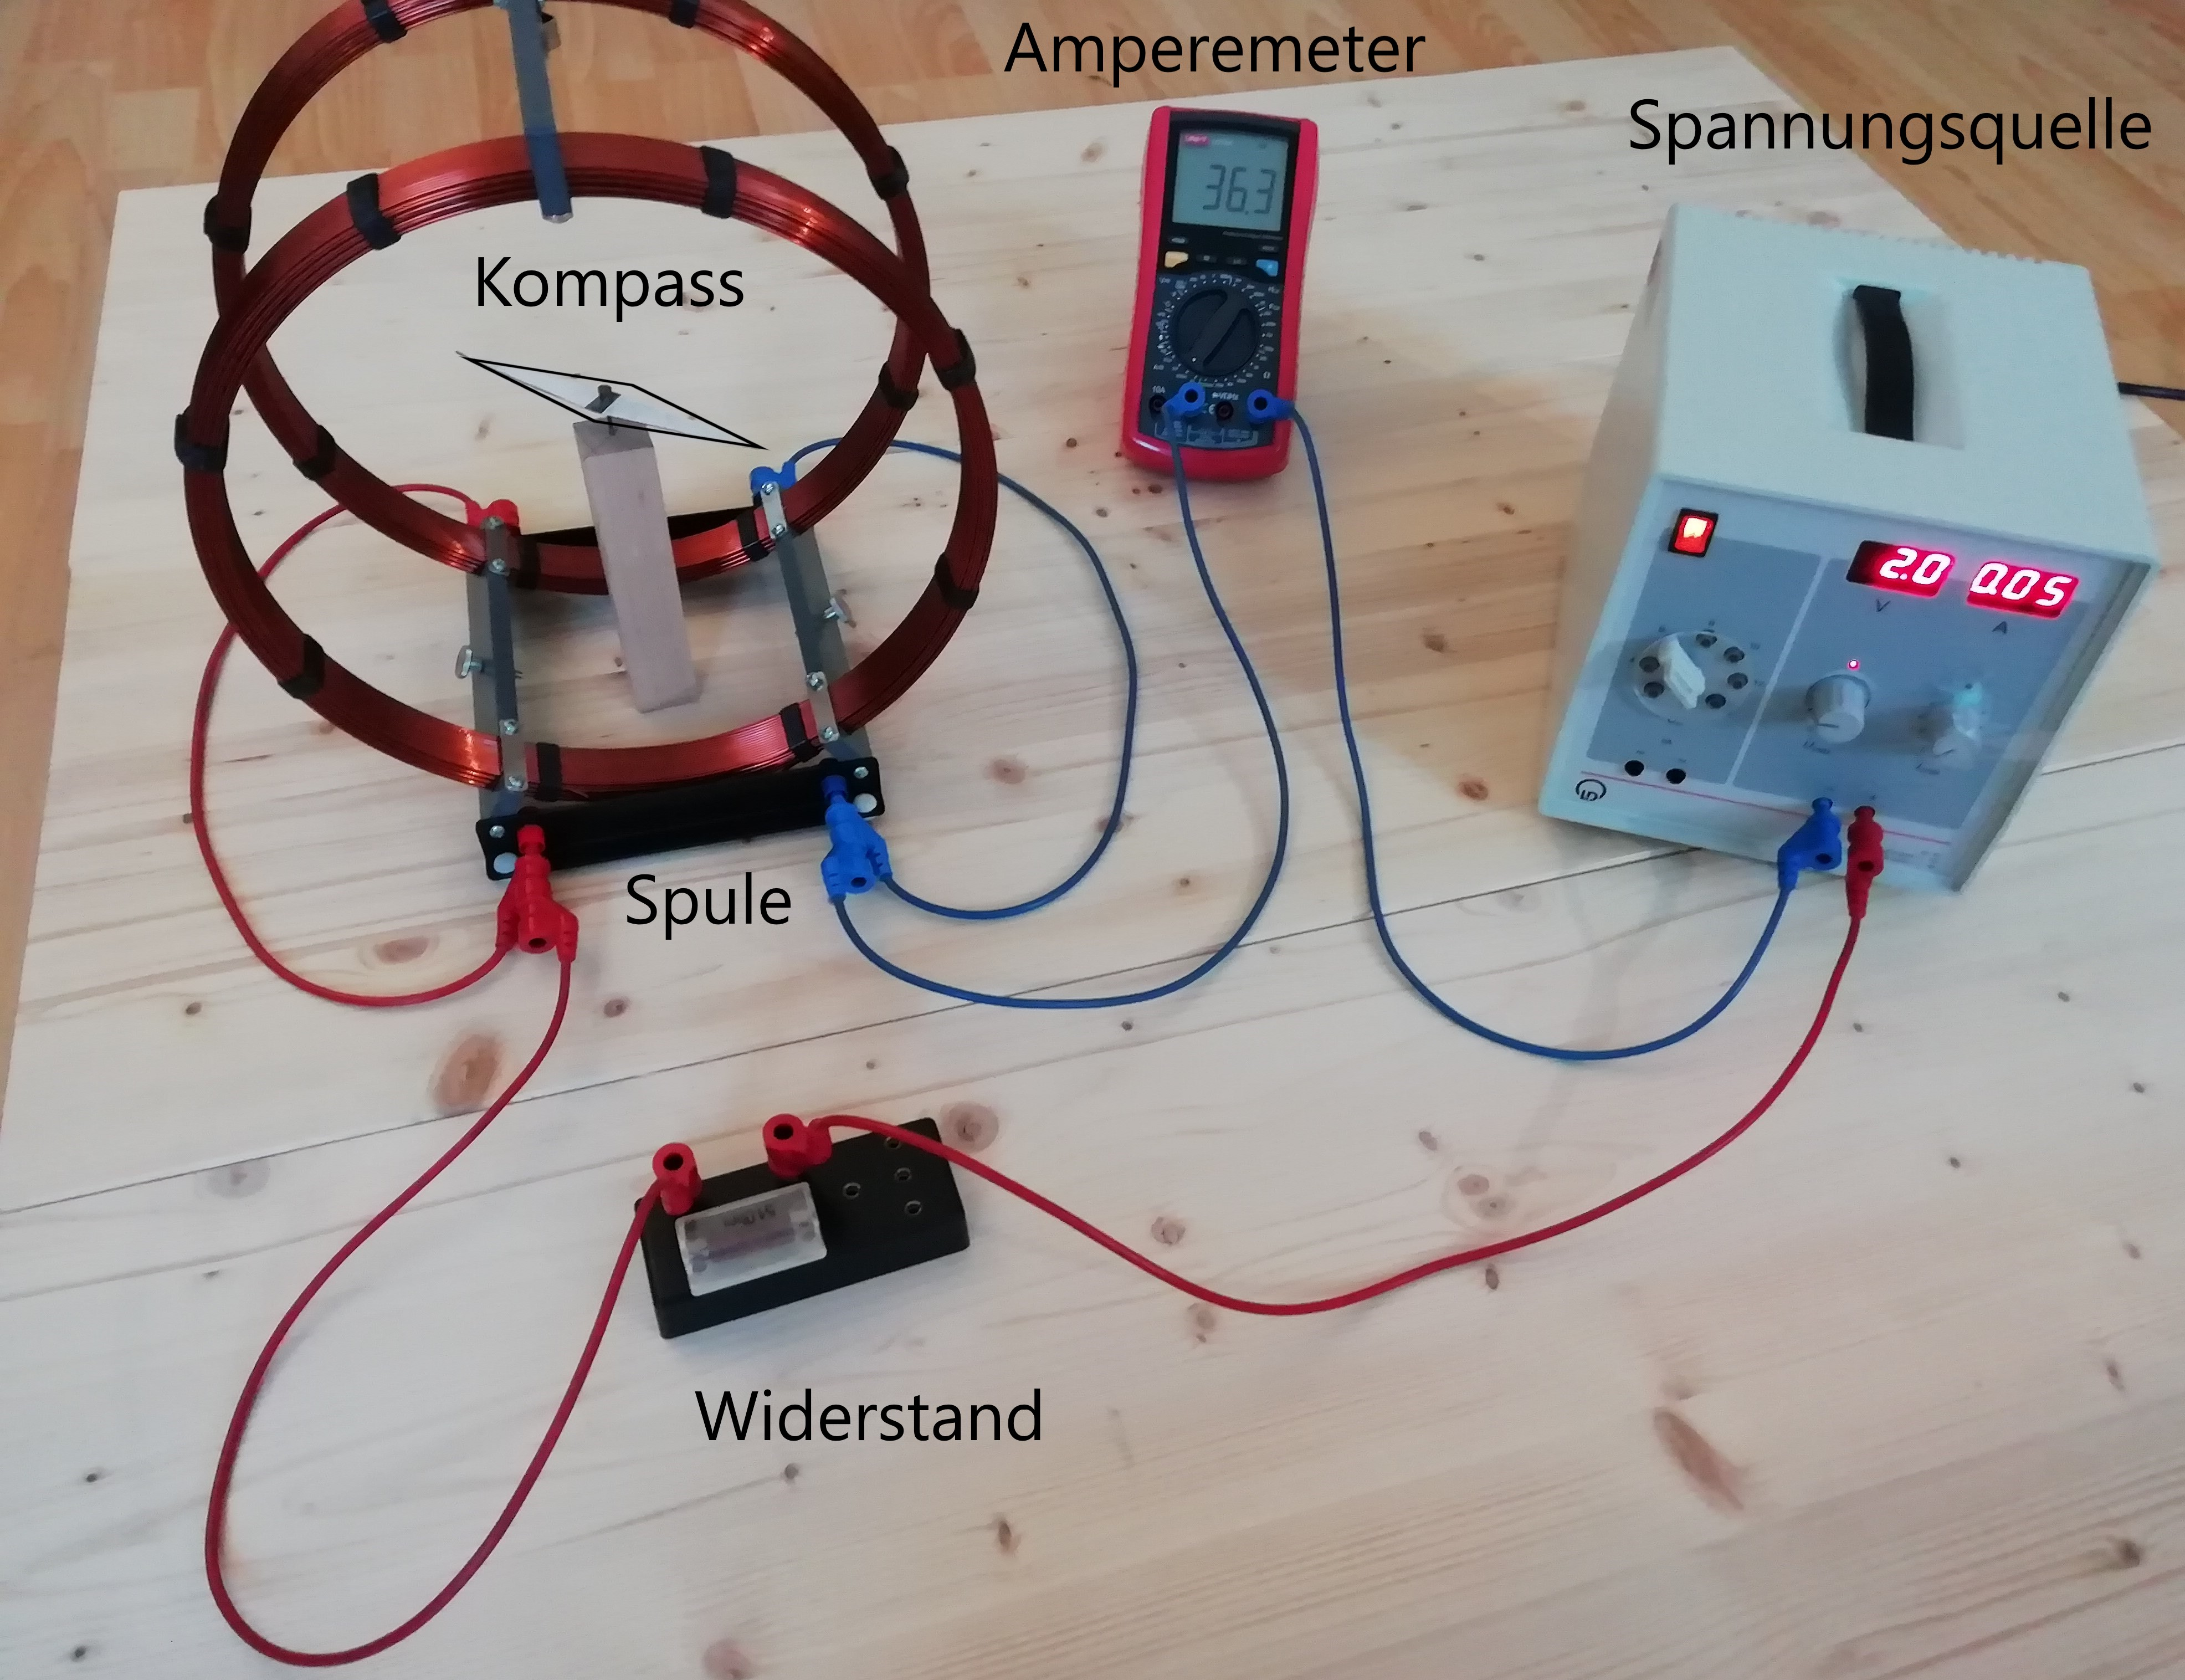
\includegraphics[width=0.9\textwidth]{images/papers/setup_labled.jpg}\\
	\small Foto des Versuchsaufbaus mit Bezeichnung der Elemente.
\end{minipage}
\end{frame}
